\chapter{Satellite Constellation Management Tools} \label{chapter_tools}
This chapter presents all the tools developed along this work to achieve the purposes of the thesis.



\section{Orbit Propagators}
Applications and topics covered by this thesis clearly require an orbital propagator to be studied.
All the propagators produced along this work exploit the Cowell's model shown in subsection \ref{orbit_prop_paragraph}.
Both undisturbed and perturbed motion have been analysed.

Orbit propagators must take in input the following data:
\begin{itemize}
    \item \textbf{Initial orbit}. The initial state of the staellite orbit must be defined before propagation.
          All the six orbital elements (see subsection \ref{sat_state_rep_paragraph}) and the epoch are required. 
          The scripts can also work defining the six components of position and velocity vectors.
          Even the TLE can be set as input, which will be appropriately converted into the classical elements representation.  
    \item \textbf{Spacecraft specifications}. According to the features of the selected propagator, one or more satellite characteristics shall be provided when considering perturbations.
          For instance, in presence of atmospheric drag, $C_D$ and $BC$ (which means cross-sectional area and mass) are needed. 
          The reflectivity coefficient must be added if the problem takes into account the SRP.
    \item \textbf{Time settings}. These input parameters include \textit{time frame} and \textit{time step}.
          The first one simply consists of the total temporal period of propagation requested by the user.
          On the other hand, the time step is strictly related to the output accuracy.
          Lower values imply more accurate results, as well as longer computation times.
          In a nutshell, the outputs will be discretized in as many points as those deriving from the ratio between time frame and time step.
          The accuracy of the model is actually always the same. 
          The difference lies in the shape of the outputs: small time steps provide narrower plots. 
          Figure \ref{time_step_fig} shows the SMA of a LEO satellite propagated for one orbit that lasts approximately 50 minutes. The assigned time step is of 5 minutes (the curve is therefore discretized into 10 points).
    \item \textbf{Perturbations parameters}. Propagators that involve any perturbing acceleration need the parameters which describe that force. 
          For example, the perturbing specific force of atmospheric drag (equation \ref{eq:drag_acc}) requires the air density, which will be given by a specific atmospheric model.
          Even for the acceleration of an eventual thruster it is necessary to specify the force it generates.
\end{itemize}

\begin{figure}[h]
      \centering
      %\textbf{Your title}\par\medskip
      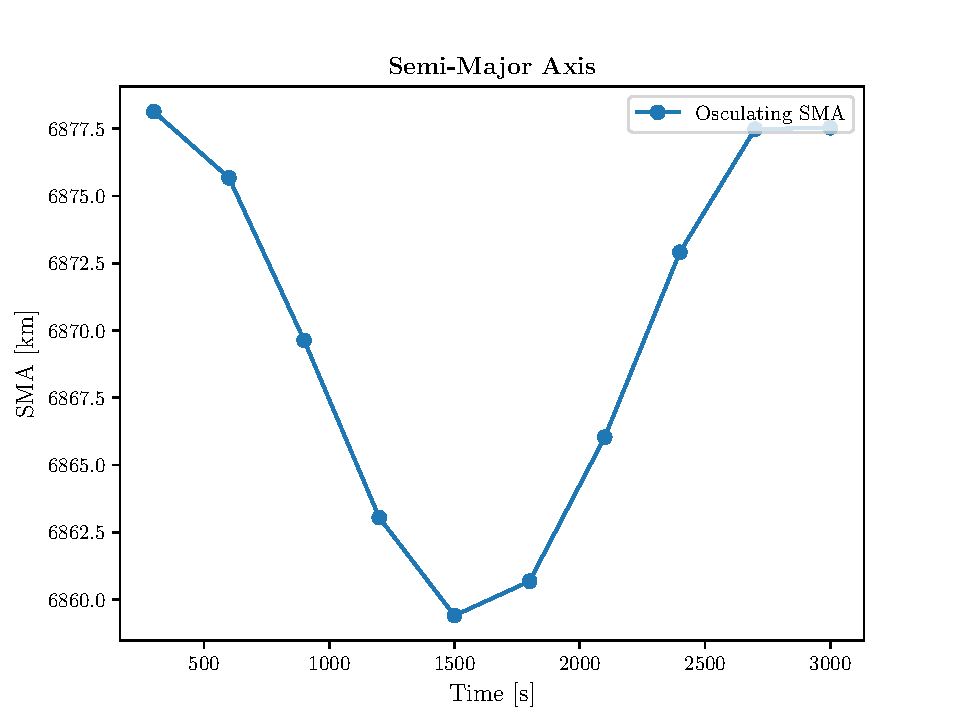
\includegraphics[scale=0.8]{img/time_step.pdf}
      \caption{Osculating SMA of a LEO satellite during one orbit. Propagation time settings: time step = 5 minutes, time frame = 50 minutes.}
      \label{time_step_fig}
  \end{figure}


\subsection{Undisturbed Motion}
The first orbit propagator proposed by this thesis consists of the ideal motion of a spacecraft neglecting all the possible perturbations that might affect it.
Therefore, this kind of propagation is governed by the two-body equation shown in subsection \ref{twobody_par}.

This model is mainly useful for two reasons.
First, it requires computation times definitely shorter than a perturbed propagation, allowing quick results when perturbations are not considered decisive for the purposes of the user.
Secondly, it provides an educational method to better understand the perturbing effects when compared to more realistic propagators.

Figure \ref{kep_low_ecc_fig} shows the orbital elements values of the motion of a satellite in LEO.
\begin{figure}[h]
      \centering
      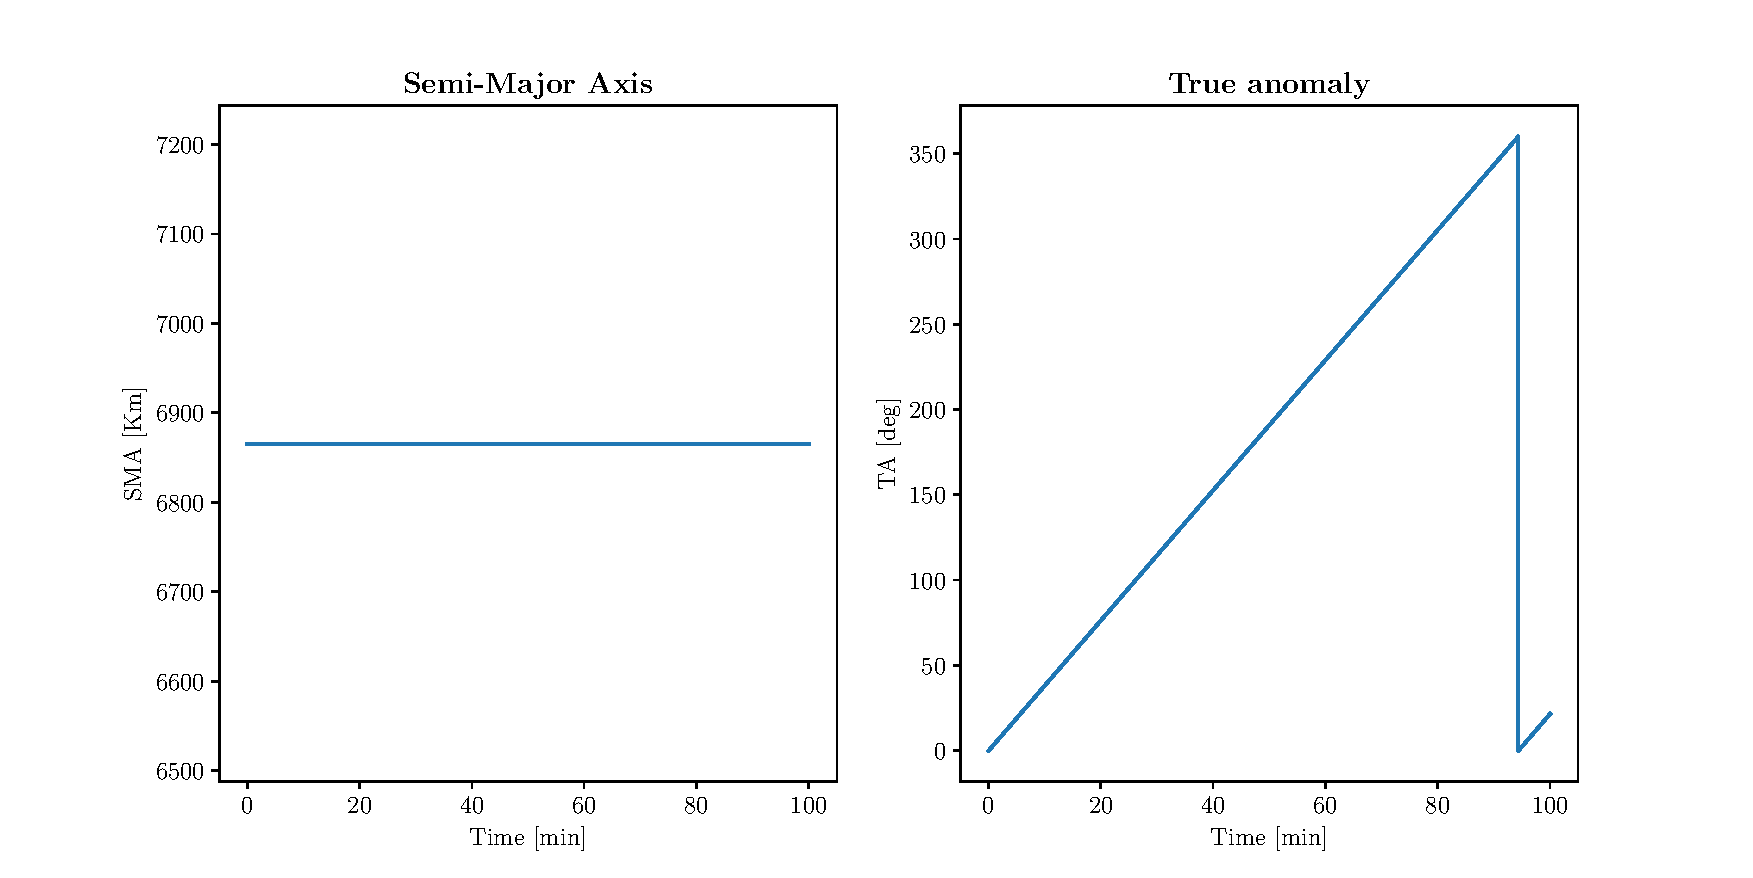
\includegraphics[scale=0.5]{img/keplerian_elements_low_ecc.pdf}
      \caption{SMA and true anomaly variation along around one LEO satellite orbit with eccentricity of 0.001}
      \label{kep_low_ecc_fig}
\end{figure}
Only SMA and true anomaly are reported for matters of layout.
The graph of the other elements is constant like the semi-major axis, because no perturbation affects their behavior.
The true anomaly is the only time-variant parameter, and in this case its curve looks like varying constantly.
The reason of this aspect lies in the eccentricity: this example is characterized by a near-circular orbit, therefore the velocity of the satellite is almost the same along the entire orbit.
Increasing the eccentricity value, like in figure \ref{kep_high_ecc_fig}, the true anomaly changes more rapidly when is in proximity of the perigee and vice-versa.
\begin{figure}[h]
      \centering
      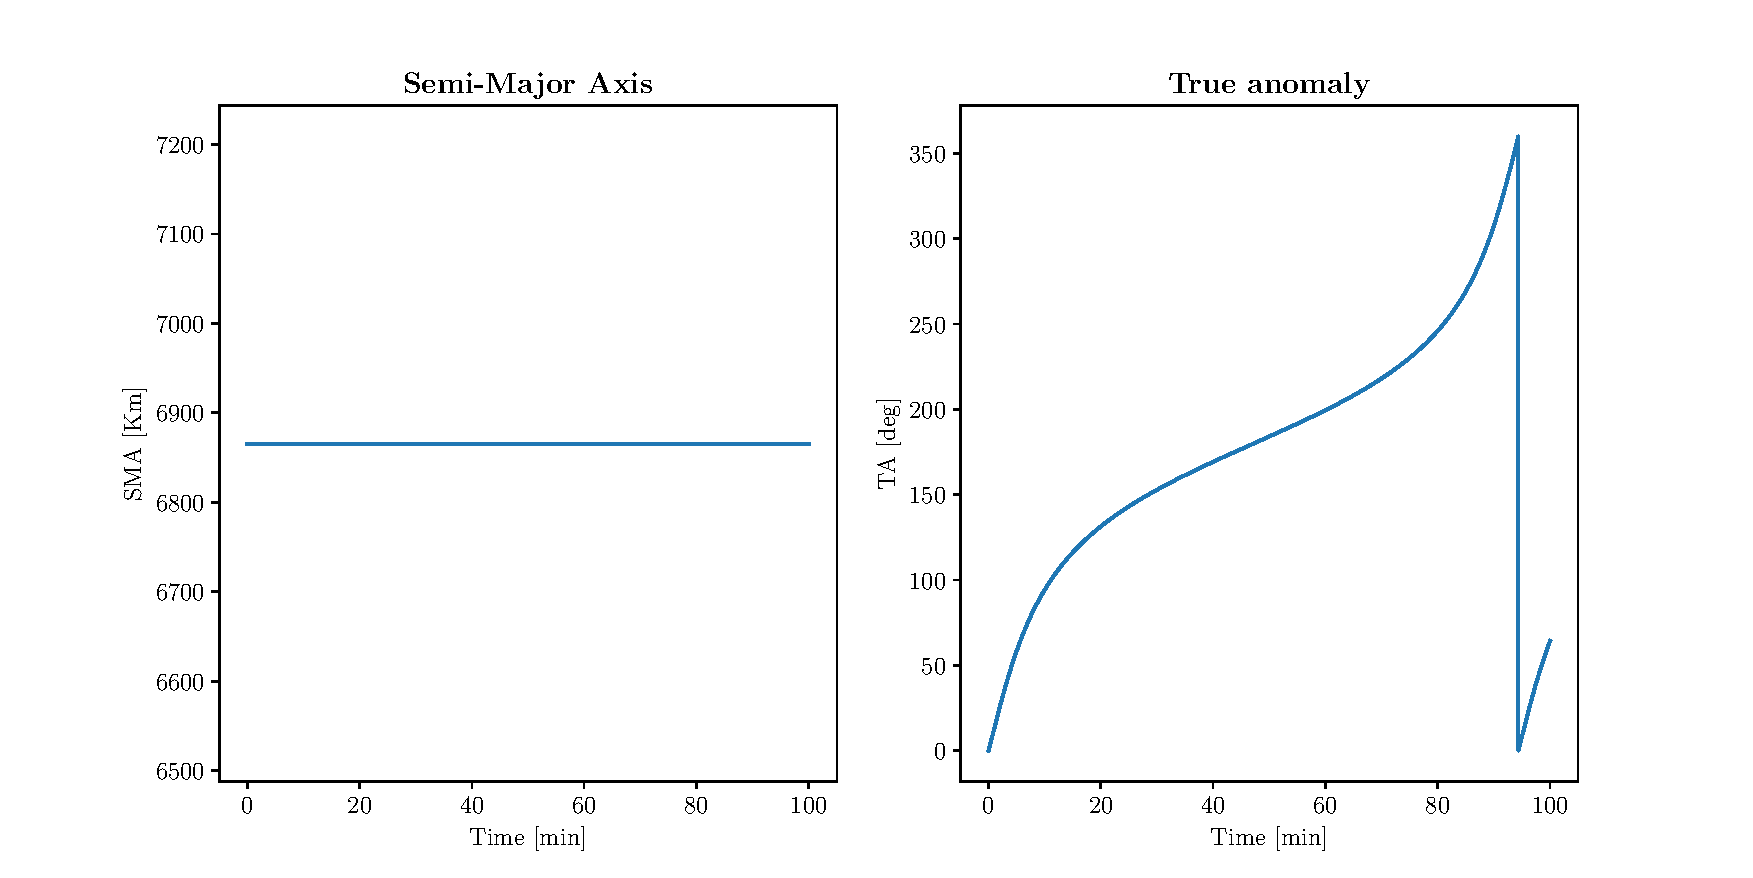
\includegraphics[scale=0.5]{img/keplerian_elements_high_ecc.pdf}
      \caption{SMA and true anomaly variation along around one LEO satellite orbit with eccentricity of 0.5}
      \label{kep_high_ecc_fig}
\end{figure}

All the case studies of this research consist of near-circular orbits.
Despite the fact that zero-eccentricity condition is not feasible, this comparison demonstrates that very low values of eccentricity make the assumption of circular orbit highly acceptable.  


\subsection{Perturbations}
The propagators developed by this work which take into account perturbing effects are based on the Cowell's technique of subsection \ref{orbit_prop_paragraph}.

Since Sun-synchronous orbits at low altitudes denote the main discussion point of this thesis, Earth's oblateness and atmospheric drag represent the perturbations of greatest interest. 
However, propagations with SRP and 3rd-body forces have been examined as well for assessing long-term effects. 

The perturbing acceleration functions performed by this thesis come from poliastro's library.

\subsection{Atmospheric Models}
Atmospheric drag exponential model has been found to be too approximate compared to the results provided by GMAT of same examples.
For that reason, two more accurate atmospheric models have been implemented into the scripts designed along this work.
The first one consists of COESA76 model, while the second is the JB2008 one.
Their theoretical background has been already exposed in paragraph \ref{orbit_prop_paragraph}.
JB2008 is definitely the most accurate model


\subsection{Mean Orbital Elements Converter}
\subsection{Sun Synchronous Orbits Functions}
\subsection{Satellite Constellation Propagator}

\section{Revisit Time Collector}

\section{Station-Keeping Simulator}

\section{Differential Drag Algorithm}